\section{Introduction}

Predictive modelling using machine learning is an effective method for building compiler heuristics, but there is a shortage of benchmarks. Typical machine learning experiments outside of the compilation field train over thousands or millions of examples. In machine learning for compilers, however, there are typically only a few dozen common benchmarks available. This limits the quality of learned models, as they have very sparse training data for what are often high-dimensional feature spaces. What is needed is a way to generate an unbounded number of training programs that finely cover the feature space. At the same time, the generated programs must be similar to the types of programs that human developers actually write, otherwise, the learning will target the wrong parts of the feature space.

This chapter introduces \emph{CLgen}, a generator for OpenCL benchmarks. Open source repositories are mined for program fragments which are used to automatically construct deep learning models for how humans write programs. The models are sampled to generate an unbounded number of runnable training programs. The quality of the programs is such that even human developers struggle to distinguish the generated programs from handwritten code. In this chapter, CLgen is used to automatically synthesise thousands of programs and show that learning over these improves the performance heterogeneous workloads using a state-of-the-art predictive model by $1.27\times$. In addition, the fine covering of the feature space automatically exposes weaknesses in the feature design which are invisible with the sparse training examples from existing benchmark suites. Correcting these weaknesses further increases workload performance by $4.30\times$.

Predictive modelling is a well-researched method for building optimisation heuristics that often exceed human experts and reduces development time~\cite{Micolet2016,Wang2014c,Magni2014,Cummins2016,Wang2009,Wen2015,Wang2010,Falch2015,Collins2012,Leather2014,Ogilvie2014a}. Figure~\ref{fig:training-a-predictive-model} shows the process by which a predictive model is constructed. A set of training programs are identified that are expected to be representative of the application domain. The programs are compiled and executed with different parameter values for the target heuristic, to determine which are the best values for each training program. Each program is also summarised by a vector of features which describe the information that is expected to be important in predicting the best heuristic parameter values. These training examples of program features and desired heuristic values are used to create a machine learning model which, when given the features from a new, unseen program, can predict good heuristic values for it.

\begin{figure}
  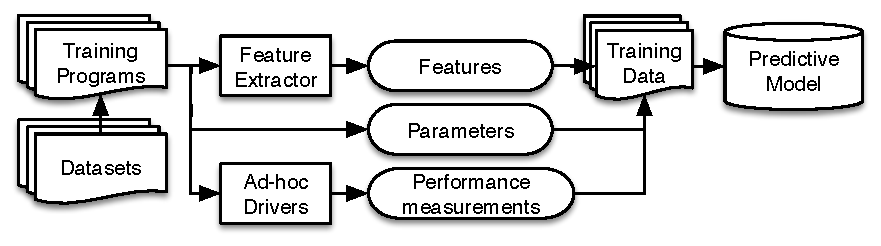
\includegraphics[width=\columnwidth]{img/overview-a}%
  \caption[Training a predictive model for compiler optimisations]{Training a predictive model for compiler optimisations. \diff{A model is constructed from training data, which comprises the features, performance measurements, and runtime parameters of training programs and their accompanying datasets.}}%
  \label{fig:training-a-predictive-model}
\end{figure}

It is common for feature vectors to contain dozens of elements. This means that a large volume of training data is needed to have adequate sampling over the feature space. Without it, the machine-learned models can only capture the coarse characteristics of the heuristic, and new programs which do not lie near to training points may be wrongly predicted. The accuracy of the machine-learned heuristic is thus limited by the sparsity of available training points.

There have been efforts to solve this problem using templates. The essence of the approach is to construct a probabilistic grammar with embedded semantic actions that define a language of possible programs. New programs may be created by sampling the grammar and, through setting probabilities on the grammar productions, the sampling is biased towards producing programs from one part of the space or another. This technique is potentially completely general since a grammar can theoretically be constructed to match any desired program domain. However, despite being theoretically possible, it is not easy to construct grammars which are both suitably general and also produce programs that are in any way similar to human-written programs. It has been shown to be successful over a highly restricted space of stencil benchmarks with little control flow or program variability~\cite{Falch2015,Cummins2016a}. But, it is not clear how much effort it will take, or even if it is possible for human experts to define grammars capable of producing human-like programs in more complex domains.

The approach introduced in this chapter does not require an expert to define what human programs look like. Instead, the structure and likelihood of programs are automatically inferred over a huge corpus of open source projects. A probability distribution is constructed over sets of characters seen in human-written code. This distribution is sampled to generate new random programs which, because the distribution models human-written code, are indistinguishable from human code. These samples can be used to populate training data with an unbounded number of human-like programs, covering the space far more finely than either existing benchmark suites or even the corpus of open source projects. The approach is enabled by two recent developments:

The first is the breakthrough effectiveness of deep learning for modelling complex structure in natural languages~\cite{Graves2013,Sutskever2014}. Deep learning is capable not just of learning the macro syntactical and semantic structure of programs, but also the nuances of how humans typically write code. It is truly remarkable when one considers that it is given no prior knowledge of the syntax or semantics of the language.

The second is the increasing popularity of public and open platforms for hosting software projects and source code. This popularity provides thousands of programming examples that are necessary to feed into the deep learning. These open source examples are not, sadly, as useful for directly learning the compiler heuristics since they are not presented in a uniform, runnable manner, nor do they typically have extractable test data. Preparing each of the thousands of open source projects to be directly applicable for learning compiler heuristics would be an insurmountable task. In addition to the program generator, CLgen, this chapter presents an accompanying host driver which generates data sets for, then executes and profiles synthesised programs.

In the course of evaluating the technique against prior work, it is discovered to be useful also for evaluating the quality of features. Since the program space is covered so much more finely than in the prior work, which only used standard benchmark suites, CLgen is able to find multiple programs with identical feature values but different best heuristic values. This indicates that the features are not sufficiently discriminative and should be extended with more information to allow those programs to be separated. Doing this significantly increases the performance of the learned heuristic. This indicates potential value of this technique for feature designers.

This chapter is organised as follows: first, Section~\ref{sec:the-case-for-benchmark-generators} presents the motivation for the use of benchmark generators in predictive modelling. Then Section~\ref{sec:clgen} introduces CLgen, a generator for human-like source code. Section~\ref{sec:cldrive} describes the driver for executing synthesised source code. CLgen is then evaluated; first through a qualitative evaluation comparing the output to handwritten code in Section~\ref{sec:clgen-qualitative-evaluation}, then quantitatively by extending the training set of a state-of-the-art machine learning optimisation heuristic. The setup of the quantitative experiments is described in Section~\ref{sec:clgen-eval-methodology}, and the results in Section~\ref{sec:clgen-eval-results}. Finally, Section~\ref{sec:clgen-conclusion} concludes this chapter.
